\documentclass[11pt]{article}

% --- Font / layout (Times-like, 11pt, single column) ---
\usepackage[margin=1in]{geometry}
\usepackage{newtxtext,newtxmath} % Times-like text + math
\usepackage{setspace}
\setstretch{1.05}

\usepackage{graphicx}
\usepackage{booktabs}
\usepackage{amsmath}
\usepackage{caption}
\usepackage{subcaption}
\usepackage{wrapfig}
\usepackage{float}
\usepackage{enumitem}
\usepackage{hyperref}
\usepackage{xcolor}
\usepackage{placeins} % enables \FloatBarrier

\graphicspath{{figs/}}

\captionsetup{font=small,labelfont=bf}
\setlist[itemize]{topsep=2pt,itemsep=2pt,parsep=0pt,partopsep=0pt,leftmargin=*}

\title{\textbf{Short-Term Stock Volatility Regime Modeling}\\
\vspace{0.15em}\large SIADS 696 Milestone II Project Report}
\author{Tanzim Chowdhury \and Tameem Syed}


\date{\vspace{-1.0em}March 2026}
\setlength{\parindent}{0pt}
% --- Paragraph spacing (readability) ---
\setlength{\parskip}{6pt}   % space between paragraphs
\setlength{\parindent}{0pt} % no indent (you already had this)

% --- Lists: indent + breathing room ---
\setlist[itemize]{
  leftmargin=1.6em,   % indent bullets (fixes "not indented")
  labelsep=0.6em,
  topsep=6pt,
  itemsep=3pt,
  parsep=2pt,
  partopsep=0pt
}

\begin{document}

% =========================
% Cover page (separate)
% =========================
\begin{titlepage}
    \centering
    \vspace*{1.2in}
    {\LARGE \textbf{Short-Term Stock Volatility Regime Modeling}\par}
    \vspace{0.35in}
    {\Large SIADS 696 Milestone II Project Report\par}
    \vspace{0.55in}
    {\large \textbf{Team Members}\par}
    \vspace{0.15in}
    {\large Tanzim Chowdhury\par}
    {\large Tameem Syed\par}

\vspace{0.6in}

{\small
Project Repository:\\
\url{https://github.com/Tanzim-Chowdhury/SIADS696-volatility-regime-modeling}
}

\vfill
{\large March 2026\par}
\end{titlepage}

% =========================
\section{Introduction}
Financial markets exhibit alternating periods of calm and turbulence. Being able to anticipate short-term shifts into higher-volatility regimes can support downstream decisions such as risk management, portfolio rebalancing, and stress testing. In this project, we model \textit{forward 5-day realized volatility regimes} (Low / Mid / High) using both supervised and unsupervised learning approaches.

Rather than attempting to forecast exact volatility values, our objective is to classify each day--asset observation into one of three interpretable volatility states. This regime-based framing allows models to focus on identifying broader market conditions rather than predicting noisy point estimates. All predictive features are constructed using information available at or before time $t$, while the target label is defined using realized volatility computed from returns over the future window $t+1 \dots t+5$. This ensures that the modeling pipeline remains strictly leakage-safe.

The main empirical findings of the study can be summarized as follows:

\begin{itemize}
\item \textbf{Supervised learning results.} Overall predictive performance is modest and sensitive to regime imbalance. Logistic Regression achieves the best test Macro F1 score ($\approx 0.466$), while a tuned HistGradientBoosting model attains slightly higher test accuracy ($\approx 0.523$) but a lower Macro F1 score ($\approx 0.451$).

\item \textbf{Unsupervised learning results.} A three-state Gaussian Hidden Markov Model (HMM) aligns with volatility regimes substantially better than K-Means clustering after mapping clusters to regimes. The HMM achieves a mapped test Macro F1 of approximately $0.543$, compared with roughly $0.393$ for K-Means.
\end{itemize}

These results suggest that while short-horizon volatility regime prediction remains challenging, incorporating temporal structure through probabilistic state models can yield stronger regime alignment than purely distance-based clustering methods.

\section{Related Work}
Volatility modeling is commonly approached using GARCH-family models, realized-volatility feature engineering, and modern ML classifiers over lagged volatility indicators. Our work is most similar to studies that (i) use realized volatility as a target signal, (ii) incorporate market-wide fear indices such as VIX as exogenous predictors, and (iii) treat market dynamics as latent regimes that can be discovered with clustering or HMMs. Relative to classic parametric models, we emphasize a reproducible feature pipeline and compare supervised vs.\ unsupervised regime recovery under a consistent, time-aware evaluation design.

\section{Data Sources and Dataset Construction}
We used daily price/volume time series for three liquid instruments: SPY, QQQ, and AAPL, spanning 2018-01-01 through 2026-02-06 (after feature construction and NA filtering, the effective date range begins 2018-03-29). We also used the CBOE Volatility Index (VIX) as a market-wide risk proxy. Raw OHLCV and VIX series were retrieved, cleaned, and merged into a unified daily dataset keyed by date; VIX values were joined onto each asset-day record to provide consistent market context.
After feature engineering and leakage-safe label construction, the final modeling table contains:
\begin{itemize}
    \item 5{,}928 rows and 30 columns (including identifiers and label),
    \item 3 tickers: AAPL, QQQ, SPY,
    \item 26 numeric feature columns used by supervised models,
    \item a 3-class regime label based on forward 5-day annualized realized volatility.
\end{itemize}

Chronological splits were fixed to mimic realistic deployment:
\begin{itemize}
    \item \textbf{Train:} through 2022-12-30
    \item \textbf{Validation:} 2023-01-03 to 2023-12-29
    \item \textbf{Test:} 2024-01-02 to 2026-02-06
\end{itemize}

\section{Feature Engineering and Label Definition}
\subsection{Log returns and realized volatility features}
We transform price into log returns for stationarity:
\[
r_t = \log(P_t) - \log(P_{t-1}).
\]
For each asset, we compute rolling realized volatility (annualized) over multiple horizons (e.g., 10, 20, 60 trading days) and include rolling volume statistics (mean/std over 10 and 20 days). To capture short memory effects, we add lagged returns:
\[
r_{t-1}, r_{t-2}, r_{t-3}, r_{t-5},
\]
and similarly include lagged VIX log returns ($1$--$3$ days) to represent market-wide shock persistence.

\subsection{Forward 5-day label (leakage-safe)}
The target signal is \textbf{forward realized volatility} over a 5-day horizon:
\[
\mathrm{RV}^{(5)}_{t,\mathrm{fwd}} = \sqrt{252}\cdot \mathrm{std}(r_{t+1}, \dots, r_{t+5}),
\]
which is assigned to date $t$ by shifting the rolling window forward. This creates a supervised learning task of predicting the \textit{future} volatility regime using only past and present information.
To form regimes, we bin $\mathrm{RV}^{(5)}_{t,\mathrm{fwd}}$ into three quantile-based categories (Low/Mid/High). Critically, the bin edges are computed \textbf{using only training-period labels} to prevent information leakage from future periods.

\begin{figure}[H]
    \centering
    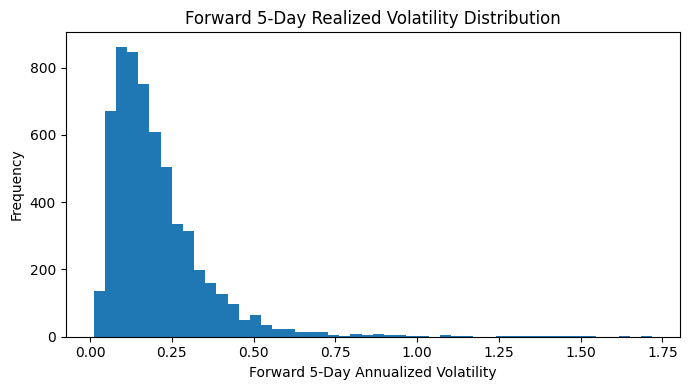
\includegraphics[width=0.78\textwidth]{fwd_rv5_distribution.png}
    \caption{Distribution of forward 5-day annualized realized volatility used to define regime bins.}
\end{figure}

Figure~1 shows the heavy right tail of forward volatility. This shape motivates a regime-based framing: the ``High'' regime is relatively rare but decision-relevant, and models must be evaluated in a way that does not let the majority ``Low/Mid'' regimes dominate the score.

\FloatBarrier

\subsection{Class balance}
Overall regime counts were approximately: Low (2241), Mid (2137), High (1550). Because the High regime is least frequent, we prioritize metrics that treat classes more evenly (Macro F1) rather than accuracy alone.

\newpage
% =========================
\section{Part A --- Supervised Learning}
\subsection{A1. Methods Description and Justification}
We trained three diverse supervised model families to satisfy the requirement for method diversity:
\begin{itemize}
    \item \textbf{Logistic Regression (probabilistic linear model)} --- an interpretable baseline to test whether the engineered features separate regimes approximately linearly.
    \item \textbf{Random Forest (bagged tree ensemble)} --- captures nonlinearities and feature interactions without heavy tuning assumptions.
    \item \textbf{HistGradientBoosting (boosted tree ensemble)} --- often strong for tabular data; sequentially fits trees to correct prior errors, but can overfit noisy financial signals unless regularized.
\end{itemize}

All supervised models share an identical preprocessing pipeline to avoid leakage and ensure comparability: \textit{median imputation} for missing values and \textit{standard scaling} for numeric features, both fit on the training split only and applied to validation/test via a scikit-learn Pipeline.

\subsection{A2. Hyperparameter Tuning: What We Changed and Why}
We explicitly tuned parameters that control \textbf{bias/variance} and \textbf{robustness to noise}, because short-horizon volatility prediction is dominated by stochasticity and regime boundaries can be ambiguous.

\paragraph{Logistic Regression tuning.}
We tuned:
\begin{itemize}
    \item \textbf{Regularization strength:} $C \in \{0.01, 0.1, 1, 10, 100\}$.
    \item \textbf{Class weighting:} \texttt{class\_weight} $\in \{\texttt{None}, \texttt{balanced}\}$.
\end{itemize}
Rationale: $C$ controls the degree of shrinkage (smaller $C$ means stronger regularization), which can improve generalization when features are correlated and noisy. Class weighting is a direct intervention for regime imbalance, intended to improve recall on the rarer High-volatility class at the possible expense of overall accuracy.

\textbf{Selected configuration (by validation Macro F1):} $C=1.0$, \texttt{class\_weight=None}. This indicates that moderate regularization worked best and explicit reweighting did not improve macro-balanced performance for this dataset.

\paragraph{HistGradientBoosting tuning.}
We tuned:
\begin{itemize}
    \item \textbf{Tree depth:} \texttt{max\_depth} (tested shallow depths; best at 3),
    \item \textbf{Leaf size:} \texttt{min\_samples\_leaf} (best at 100),
    \item \textbf{Learning rate:} \texttt{learning\_rate} (best at 0.1),
    \item \textbf{Number of boosting iterations:} \texttt{max\_iter} (best at 200).
\end{itemize}
Rationale: boosted trees can chase noise in financial series; depth and leaf size act as structural regularizers. A shallower tree (smaller depth) and larger leaf size reduce variance and encourage broader, more stable splits. Learning rate and iteration count trade off optimization speed vs.\ overfitting risk.

\textbf{Selected configuration (by validation Macro F1):}
\[
\texttt{max\_depth}=3,\quad \texttt{min\_samples\_leaf}=100,\quad \texttt{learning\_rate}=0.1,\quad \texttt{max\_iter}=200.
\]
This choice reflects a regularized boosting model designed to generalize rather than memorize.

\paragraph{Random Forest (baseline only).}
Random Forest is included as a third model family; in our final comparison it is treated as a \textbf{baseline configuration} rather than a tuned best-in-family model. We include it to test whether bagging-based nonlinearity improves the task relative to Logistic Regression and boosted trees.

\subsection{A3. Cross-Validation for Temporal Robustness (TimeSeriesSplit)}
Because this is time-series data, we cannot use random $k$-fold CV. Instead, we applied a 5-fold expanding-window TimeSeriesSplit on the training period. Each fold trains on earlier dates and validates on the subsequent time block, preserving chronology and preventing look-ahead bias.

We report mean and standard deviation of Macro F1 across folds for the supervised families that were cross-validated:
\begin{itemize}
    \item \textbf{LogReg baseline:} mean Macro F1 = 0.524, std = 0.061
    \item \textbf{HGB baseline:} mean Macro F1 = 0.455, std = 0.046
\end{itemize}
Interpretation: Logistic Regression has higher average performance across historical subperiods, suggesting that much of the predictive structure captured by our engineered features may be approximately linear and relatively stable in earlier windows. Meanwhile, HGB exhibits slightly lower fold variance, consistent with stronger regularization, but does not exceed the linear baseline on average.

\subsection{A4. Hold-out Performance and Model Comparison}
We evaluate on validation (2023) and held-out test (2024--2026) using:
\begin{itemize}
    \item \textbf{Accuracy} for overall correctness,
    \item \textbf{Macro F1} as the primary metric to balance performance across Low/Mid/High regimes.
\end{itemize}

\begin{figure}[H]
    \centering
    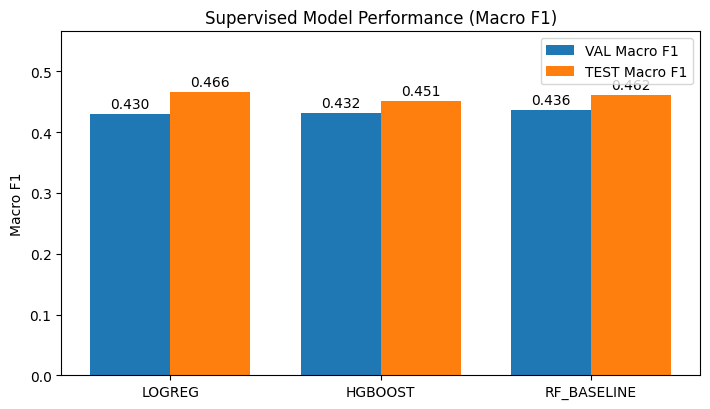
\includegraphics[width=0.86\textwidth]{sup_model_macroF1_bar.png}
    \caption{Supervised comparison (Macro F1) on validation and test.}
\end{figure}

Figure~2 shows that test Macro F1 values are close across models (roughly 0.45--0.47), reinforcing that the task is intrinsically difficult. Logistic Regression attains the best test Macro F1 ($\approx$0.466), while tuned HGB slightly improves accuracy but not Macro F1. The Random Forest baseline performs comparably, suggesting that tree-based nonlinearities provide limited gain over the linear baseline given the current feature set and short prediction horizon.

\subsection{A5. Confusion Matrices and Error Structure}
To understand \textit{how} the models fail, we examine test confusion matrices. We focus on systematic patterns rather than isolated counts.

\begin{figure}[H]
\centering
\begin{subfigure}{0.31\textwidth}
    \centering
    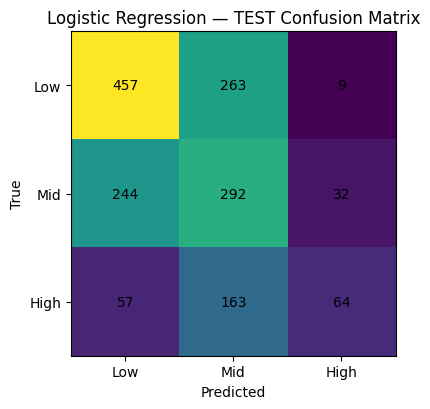
\includegraphics[width=\textwidth]{cm_test_logreg.png}
    \caption{LogReg (Test)}
\end{subfigure}\hfill
\begin{subfigure}{0.31\textwidth}
    \centering
    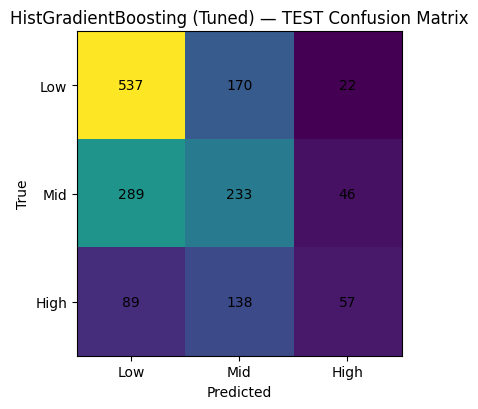
\includegraphics[width=\textwidth]{cm_test_hgboost.png}
    \caption{HGB Tuned (Test)}
\end{subfigure}\hfill
\begin{subfigure}{0.31\textwidth}
    \centering
    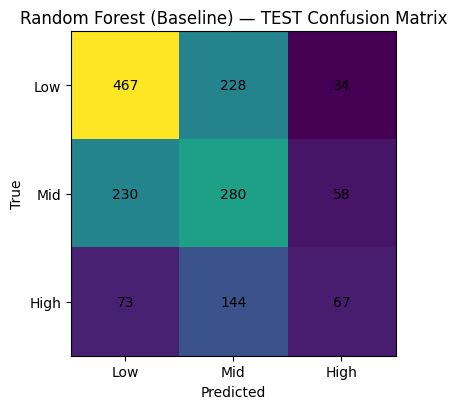
\includegraphics[width=\textwidth]{cm_test_rf.png}
    \caption{RF Baseline (Test)}
\end{subfigure}
\caption{Test confusion matrices for supervised models.}
\end{figure}

Across models, the most common errors are \textbf{adjacent-regime confusions} (Low$\leftrightarrow$Mid and Mid$\leftrightarrow$High), which is expected because regimes are defined by quantile thresholds on a continuous volatility signal. In particular, the High regime is frequently predicted as Mid, indicating that extreme volatility is hard to distinguish from moderately elevated volatility using only lagged features. This aligns with domain intuition: abrupt transitions into volatility spikes often reflect exogenous shocks not encoded in a small set of recent-day indicators.

\subsection{A6. Sensitivity Analysis (HGB Hyperparameters)}
We performed sensitivity analysis for HistGradientBoosting by measuring validation Macro F1 across a grid of \texttt{max\_depth} and \texttt{min\_samples\_leaf}. This goes beyond simply selecting a ``best'' configuration by testing stability across nearby settings.

\begin{figure}[H]
    \centering
    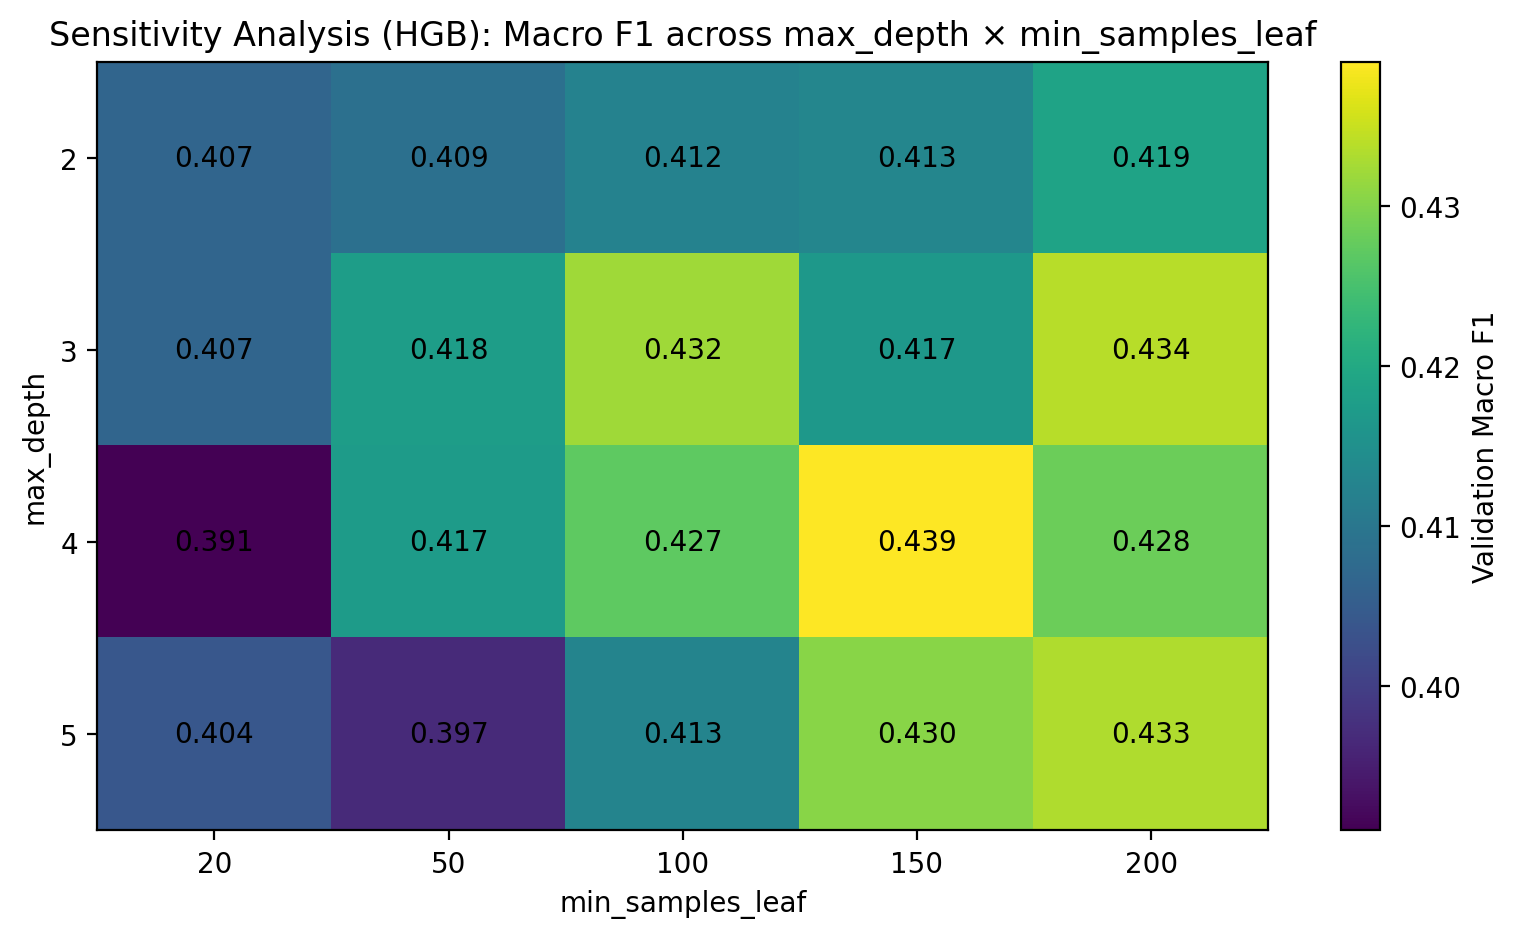
\includegraphics[width=0.88\textwidth]{sup_sensitivity.png}
    \caption{Sensitivity Analysis (HGB): validation Macro F1 across \texttt{max\_depth} $\times$ \texttt{min\_samples\_leaf}.}
\end{figure}

Figure~4 indicates that performance varies meaningfully across the grid, but the strongest region occurs around \texttt{max\_depth}=3 with mid-to-large leaf sizes (notably \texttt{min\_samples\_leaf}$\approx$100). This supports our design choice to regularize boosting: deeper trees and very small leaves can overfit short-term noise and degrade Macro F1, while overly aggressive leaf sizes can underfit. The chosen tuned parameters lie in a relatively robust ``plateau'' rather than a fragile, single-point optimum.

\subsection{A7. Feature Ablation: Asset-only vs VIX-only vs Full}
To understand which feature groups contribute most, we compare validation Macro F1 under three feature sets:
\begin{itemize}
    \item \textbf{FULL (26 features)}: asset + volume + VIX features
    \item \textbf{ASSET\_ONLY (18 features)}: asset/volume only (removing VIX block)
    \item \textbf{VIX\_ONLY (8 features)}: VIX features only (removing asset block)
\end{itemize}

Key results (validation Macro F1):
\begin{itemize}
    \item LogReg: FULL 0.430 $\rightarrow$ ASSET\_ONLY 0.385 $\rightarrow$ VIX\_ONLY 0.336
    \item HGB Tuned: FULL 0.432 $\rightarrow$ ASSET\_ONLY 0.403 $\rightarrow$ VIX\_ONLY 0.392
\end{itemize}

Interpretation: the \textbf{full feature set is best} for both models. VIX-only features are insufficient for the linear model, indicating that regime separation benefits from asset-specific realized volatility and volume context. Interestingly, HGB maintains relatively stronger performance on VIX-only than LogReg, consistent with the idea that nonlinear models can extract more structure from compact exogenous signals, though still not outperforming the full feature representation. Overall, this ablation supports the hypothesis that both \textbf{market-wide risk} (VIX) and \textbf{asset-local dynamics} are jointly necessary for best regime prediction.

% =========================
% UPDATED SECTION (A8) ONLY
% =========================
\subsection{A8. Failure Analysis (Quantitative + Categories)}
We analyzed failures using the saved prediction tables and computed two complementary error summaries: (i) \textbf{error rate} (1 -- accuracy) and (ii) \textbf{mean absolute error (MAE)} in ordinal regime space, where regimes are encoded as Low=0, Mid=1, High=2. MAE is useful because it distinguishes being ``off by one'' (e.g., Low$\rightarrow$Mid) from being ``off by two'' (Low$\rightarrow$High).

\paragraph{Overall failure rates.}
All three supervised models fail at broadly similar rates, reinforcing that regime prediction at a 5-day horizon is inherently noisy:
\begin{itemize}
    \item \textbf{Validation error rate:} LogReg 0.469, HGB (tuned) 0.481, RF (baseline) 0.487.
    \item \textbf{Test error rate:} HGB (tuned) 0.477, RF (baseline) 0.485, LogReg 0.486.
\end{itemize}
While the ranking shifts slightly between validation and test, differences are modest (on the order of 1--2\%), suggesting that model family changes alone do not fundamentally solve the task.

\paragraph{Error severity (ordinal MAE).}
MAE indicates most mistakes are close in regime distance:
\begin{itemize}
    \item \textbf{Validation MAE:} LogReg 0.497, HGB (tuned) 0.515, RF (baseline) 0.525.
    \item \textbf{Test MAE:} LogReg 0.528, HGB (tuned) 0.547, RF (baseline) 0.553.
\end{itemize}
MAE values near 0.5 imply that errors are frequently one-step confusions rather than extreme misclassifications, consistent with threshold-based regime labels on a continuous volatility signal.

\paragraph{Dominant misclassification patterns.}
Across models, the largest error modes are adjacent-regime confusions, especially involving the Mid regime:
\begin{itemize}
    \item \textbf{Low$\rightarrow$Mid and Mid$\rightarrow$Low} dominate: e.g., LogReg has 263 Low$\rightarrow$Mid and 244 Mid$\rightarrow$Low on test; HGB has 170 Low$\rightarrow$Mid and 289 Mid$\rightarrow$Low; RF has 228 Low$\rightarrow$Mid and 230 Mid$\rightarrow$Low.
    \item \textbf{High$\rightarrow$Mid} is also common (test counts: LogReg 163; HGB 138; RF 144), reflecting that extreme volatility is frequently softened into the Mid regime.
    \item Two-step errors (Low$\leftrightarrow$High) occur less often (e.g., test Low$\rightarrow$High counts: LogReg 9, HGB 22, RF 34), indicating the models rarely confuse calm periods with extreme turbulence directly.
\end{itemize}

\paragraph{Failure categories and interpretation.}
These quantitative patterns align with three qualitative categories:
\begin{itemize}
    \item \textbf{Boundary ambiguity:} Because regimes are defined by training-quantile thresholds, observations near bin edges are intrinsically hard to label; models are often ``wrong'' by a narrow margin, producing one-step MAE errors.
    \item \textbf{Shock-driven spikes:} High-volatility episodes driven by news or sudden liquidity events may not be predictable from short lag windows, leading to High$\rightarrow$Mid under-prediction.
    \item \textbf{Cross-asset heterogeneity:} A given VIX level may correspond to different realized volatility dynamics in SPY vs AAPL; a single pooled model can misgeneralize across instruments without asset-specific calibration.
\end{itemize}

\paragraph{Implications for next steps.}
Given that most failures are concentrated in Mid-boundary confusions, improvements are more likely to come from (i) richer exogenous covariates (macro/event features), (ii) longer-memory temporal models (sequence features / LSTM / transformer), or (iii) reframing the label (e.g., smoothing or using probabilistic regime definitions) rather than swapping between standard tabular model families.

\subsection{A9. Tradeoffs}
Our evaluation highlights key tradeoffs:
\begin{itemize}
    \item \textbf{Accuracy vs Macro F1:} tuned HGB improves accuracy slightly but does not improve Macro F1, suggesting it may be optimizing majority-class correctness rather than balanced regime detection.
    \item \textbf{Model complexity vs stability:} linear LogReg is simpler and performs competitively; increasing complexity yields limited gains given noise and short horizons.
    \item \textbf{Interpretability vs flexibility:} LogReg offers interpretable coefficients and clearer failure reasoning, while boosted trees can model nonlinearities but require careful regularization and sensitivity checks.
\end{itemize}

\newpage
% =========================
\section{Part B --- Unsupervised Learning}
\subsection{B1. Methods Description and Justification}
Unsupervised learning addresses a different question: \textit{do latent states discovered from observed market variables align with the forward-volatility regimes we defined?} We evaluate two distinct unsupervised families:
\begin{itemize}
    \item \textbf{K-Means clustering} --- a non-probabilistic baseline that partitions standardized observations into $k$ clusters by minimizing within-cluster variance.
    \item \textbf{Gaussian Hidden Markov Model (HMM)} --- a probabilistic state-space model that explicitly models temporal dependence via a Markov transition matrix and Gaussian emissions.
\end{itemize}

We fit both methods using an interpretable observation set for SPY:
\[
[\texttt{log\_return},\ \texttt{rv\_10},\ \texttt{vix\_close}],
\]
standardized using training data only. Because cluster/state IDs are arbitrary, we map clusters/states to regimes using a best-match assignment based on validation data (then apply the mapping to test).

\subsection{B2. Evaluation Metrics: ARI/NMI + Mapped Classification Scores}
We report both:
\begin{itemize}
    \item \textbf{ARI/NMI} (Adjusted Rand Index / Normalized Mutual Information) to quantify agreement between unsupervised assignments and regimes without requiring label semantics.
    \item \textbf{Mapped Accuracy / Macro F1} after mapping each cluster/state to a regime label for interpretability.
\end{itemize}
This combined view is important: a model can produce stable clusters that do not correspond to the forward-volatility label definition, and ARI/NMI help diagnose that disconnect.

\subsection{B3. K-Means Results and Interpretation}
K-Means yields limited alignment with regimes:
\begin{itemize}
    \item Validation ARI/NMI $\approx$ 0.054 / 0.053; mapped validation Macro F1 $\approx$ 0.318.
    \item Test ARI/NMI $\approx$ 0.158 / 0.097; mapped test Macro F1 $\approx$ 0.393.
\end{itemize}

\begin{figure}[H]
\centering
\begin{subfigure}{0.56\textwidth}
    \centering
    \includegraphics[width=\textwidth]{kmeans_state_timeline.png}
    \caption{K-Means cluster assignments over time (SPY).}
\end{subfigure}\hfill
\begin{subfigure}{0.40\textwidth}
    \centering
    \includegraphics[width=\textwidth]{kmeans_state_vs_regime_heatmap.png}
    \caption{K-Means vs regime (Test).}
\end{subfigure}
\caption{K-Means temporal behavior and alignment with regimes.}
\end{figure}

Interpretation: K-Means is sensitive to scale and outliers and does not encode temporal persistence. As a result, cluster switching can be frequent and may reflect day-to-day noise rather than meaningful regime transitions. The heatmap indicates that one dominant cluster absorbs much of Low/Mid, limiting separability of the High regime.

\subsection{B4. HMM Results and Interpretation}
The Gaussian HMM better captures regime structure:
\begin{itemize}
    \item Converged in 44 iterations.
    \item Validation ARI/NMI $\approx$ 0.193 / 0.126; mapped validation Macro F1 $\approx$ 0.466.
    \item Test ARI/NMI $\approx$ 0.164 / 0.105; mapped test Macro F1 $\approx$ 0.543.
\end{itemize}

\begin{figure}[H]
\centering
\begin{subfigure}{0.38\textwidth}
    \centering
    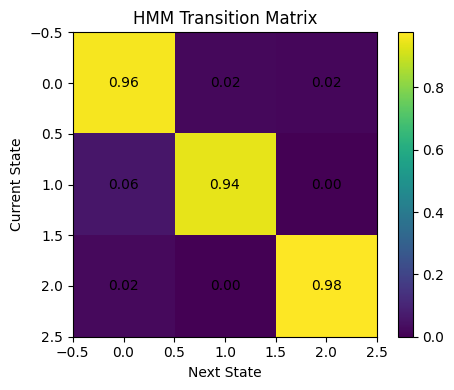
\includegraphics[width=\textwidth]{hmm_transition_matrix.png}
    \caption{Estimated transition matrix.}
\end{subfigure}\hfill
\begin{subfigure}{0.60\textwidth}
    \centering
    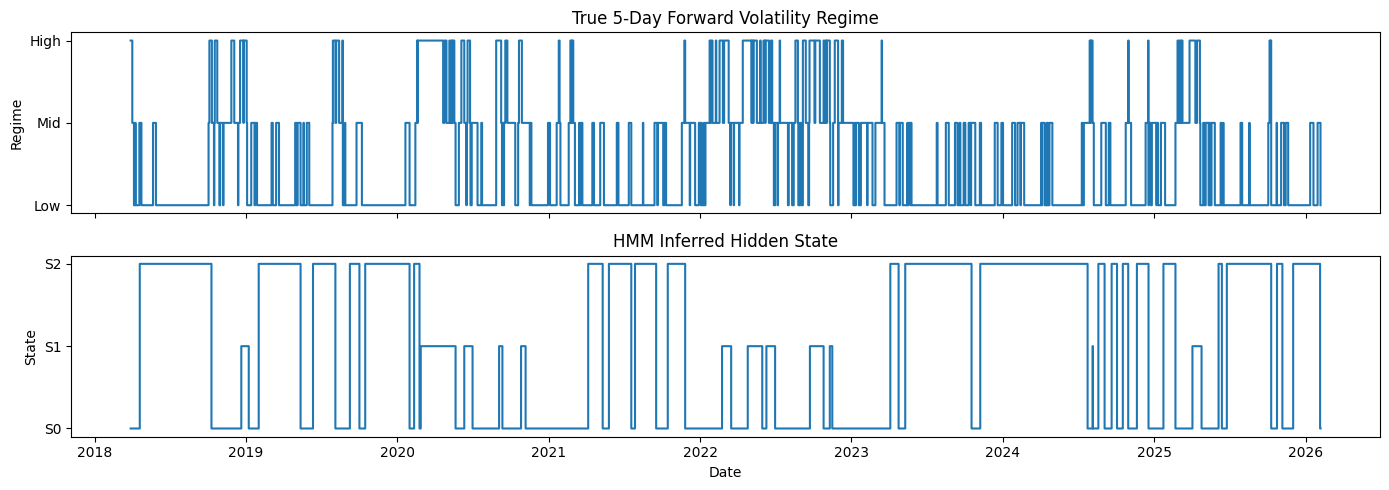
\includegraphics[width=\textwidth]{hmm_true_vs_state_timeline.png}
    \caption{True regime vs inferred HMM state (SPY).}
\end{subfigure}
\caption{HMM dynamics: persistence + alignment with regimes.}
\end{figure}

Interpretation: the transition matrix shows strong diagonal probability (state persistence), consistent with volatility clustering in finance. The timeline comparison suggests the HMM tracks extended calm vs turbulent periods more smoothly than K-Means, which matches the conceptual definition of a ``regime.'' Importantly, HMM performance improves substantially on mapped Macro F1 compared to K-Means, supporting the value of explicitly modeling temporal dependence.

\subsection{B5. Unsupervised Comparison and Sensitivity}
We summarize the mapped Macro F1 comparison and examine sensitivity to the number of clusters/states.

\begin{figure}[H]
\centering
\begin{subfigure}{0.49\textwidth}
    \centering
    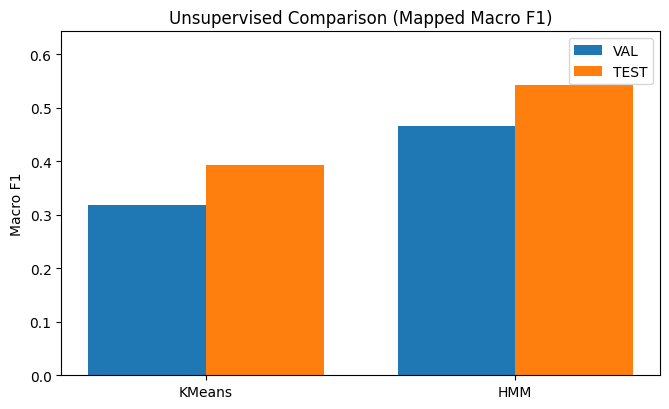
\includegraphics[width=\textwidth]{unsup_macroF1_bar.png}
    \caption{Mapped Macro F1 comparison.}
\end{subfigure}\hfill
\begin{subfigure}{0.49\textwidth}
    \centering
    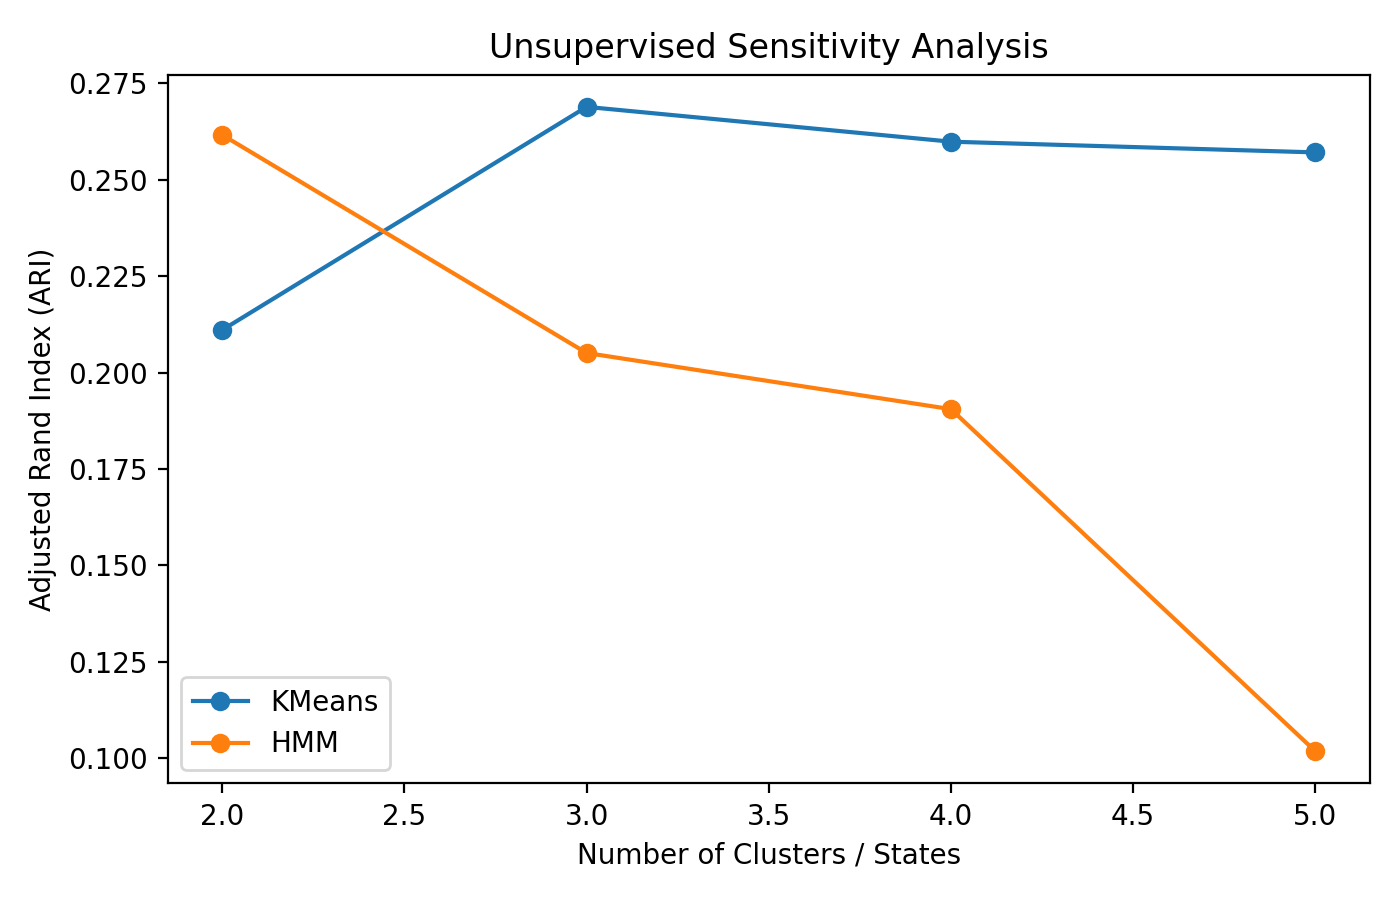
\includegraphics[width=\textwidth]{unsup_sensitivity.png}
    \caption{Sensitivity vs number of clusters/states (ARI).}
\end{subfigure}
\caption{Unsupervised results summary and sensitivity.}
\end{figure}

The sensitivity curve indicates that K-Means ARI peaks around $k=3$--$5$ with relatively small differences, while HMM ARI degrades notably as the number of states increases beyond 3. This supports selecting \textbf{3 states} for HMM as a parsimonious representation: adding more states may fragment the latent process into unstable micro-states that do not correspond to the forward-volatility regime definition.

\newpage
% =========================
\section{Discussion}
\subsection{What we learned from Part A (Supervised)}
The strongest theme is that short-horizon regime prediction is noisy: even with VIX and multi-window realized volatility features, Macro F1 remains in the mid-0.4s. Logistic Regression performing competitively suggests that (for this feature set and horizon) nonlinear models do not unlock substantial additional predictive structure. Feature ablation indicates that both local (asset) and market-wide (VIX) signals matter, and that boosted trees can make somewhat stronger use of VIX-only information than linear models.

\subsection{What we learned from Part B (Unsupervised)}
Modeling temporal structure explicitly matters. K-Means provides a baseline partition of the observation space but fails to encode persistence, producing frequent switching and weaker regime alignment. The HMM produces a more realistic depiction of regime persistence and achieves notably stronger mapped Macro F1.

\subsection{Challenges and responses}
Key challenges included leakage risk (forward labels), non-i.i.d.\ evaluation requirements, and instability of short-horizon signals across market periods. We responded by enforcing leakage-safe labeling, using strict chronological splits, adding time-series cross-validation for robustness, and incorporating sensitivity/ablation analyses to produce insight beyond raw metrics.

\subsection{Extensions}
With more time, we would (i) incorporate richer macro/exogenous covariates (rates, inflation proxies, event flags), (ii) evaluate sequence models (LSTM or temporal transformers) to capture longer memory and abrupt transitions, and (iii) explore multi-asset modeling strategies that allow partial pooling while respecting cross-asset heterogeneity.

\section{Team Contributions}
Tanzim Chowdhury led development of the data pipeline, feature engineering implementation, modeling code structure, and reproducible experimentation workflow. Tameem Syed led analysis design and visualization production, including evaluation plots, sensitivity figures, and interpretation of results. Both team members contributed to report writing, editing, and narrative integration.

% =========================
% REFERENCES (updated)
% =========================
\newpage

\begin{thebibliography}{99}
\setlength{\itemsep}{2pt}

\bibitem{engle1982}
Engle, R. F. (1982).
Autoregressive conditional heteroskedasticity with estimates of the variance of UK inflation.
\textit{Econometrica, 50}(4), 987--1007.

\bibitem{andersen2003}
Andersen, T. G., Bollerslev, T., Diebold, F. X., \& Labys, P. (2003).
Modeling and forecasting realized volatility.
\textit{Econometrica, 71}(2), 579--625.

\bibitem{hamilton1989}
Hamilton, J. D. (1989).
A new approach to the economic analysis of nonstationary time series and the business cycle.
\textit{Econometrica, 57}(2), 357--384.

\bibitem{rabiner1989}
Rabiner, L. R. (1989).
A tutorial on hidden Markov models and selected applications in speech recognition.
\textit{Proceedings of the IEEE, 77}(2), 257--286.

\bibitem{pedregosa2011}
Pedregosa, F., Varoquaux, G., Gramfort, A., Michel, V., Thirion, B., Grisel, O., et al. (2011).
Scikit-learn: Machine learning in Python.
\textit{Journal of Machine Learning Research, 12}, 2825--2830.

\bibitem{yahoo}
Yahoo Finance API.
Financial market data source used for OHLCV time series.
(Accessed 2026).

\bibitem{cboe}
Cboe Global Markets.
CBOE Volatility Index (VIX) historical data.
(Accessed 2026).

\bibitem{kaggle}
Kaggle.
Two Sigma Financial Modeling Challenge.
\textit{Kaggle Competition Dataset}.
(Accessed 2026).

\end{thebibliography}

\end{document}